\section{Analyse des paramètres des fonctions de magnitude}
\subsection{Analyse de $m_1(x,y)$}
\begin{figure}[!h]
   \begin{subfigure}[c]{.5\linewidth}
     \centering
     
\includegraphics[scale=0.35]{Chapters/Images/synthetic_map.png}
     \caption{}
   \end{subfigure} 
   \begin{subfigure}[c]{.5\linewidth}
     \centering
     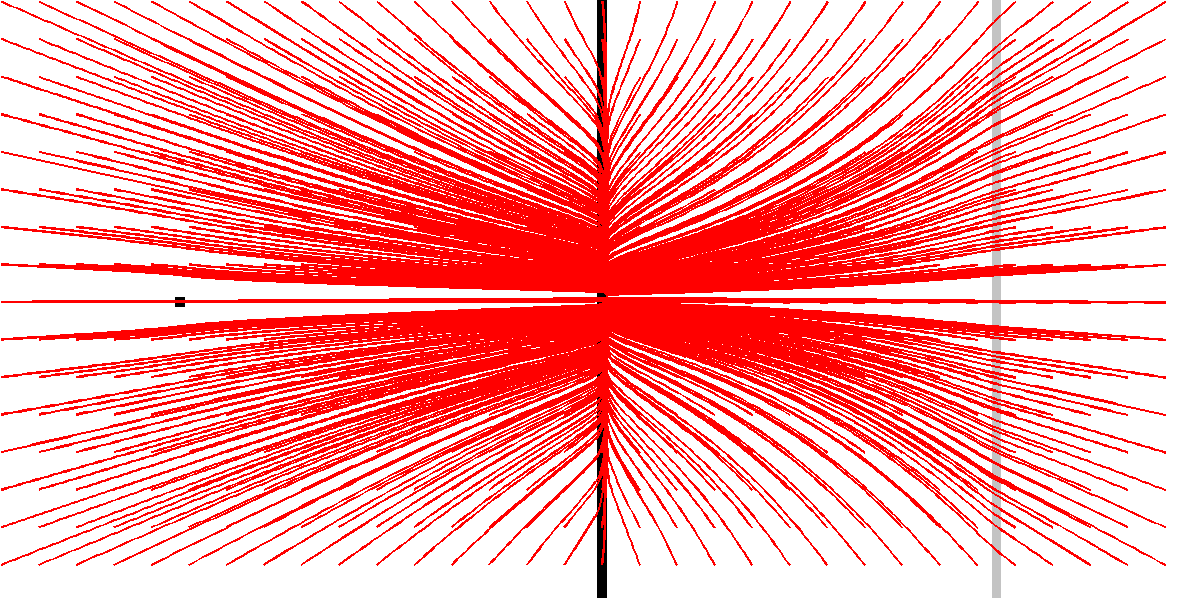
\includegraphics[scale=0.35]{Chapters/Images/m1_gamma_5.png}
     \caption{$\gamma=0.5$}
   \end{subfigure} \\
   
   \begin{subfigure}[c]{.5\linewidth}
     \centering
     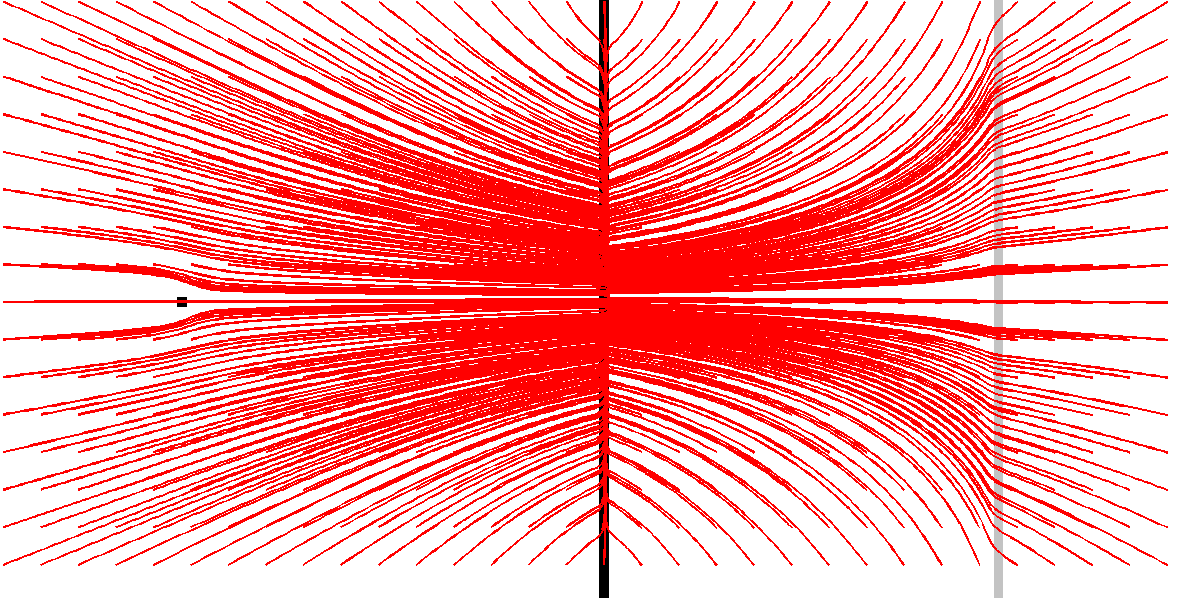
\includegraphics[scale=0.35]{Chapters/Images/m1_gamma_10.png}
     \caption{$\gamma=1.0$}
   \end{subfigure}
   \begin{subfigure}[c]{.5\linewidth}
     \centering
     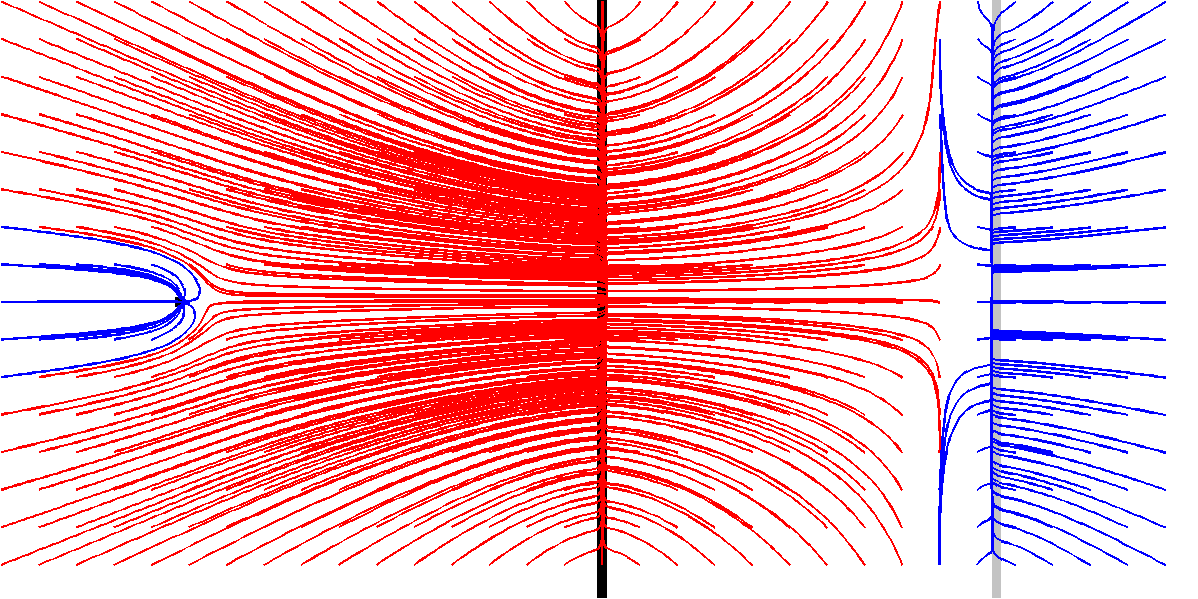
\includegraphics[scale=0.35]{Chapters/Images/m1_gamma_15.png}
     \caption{$\gamma=1.5$}
   \end{subfigure}\\
   
   \begin{subfigure}[c]{.5\linewidth}
     \centering
     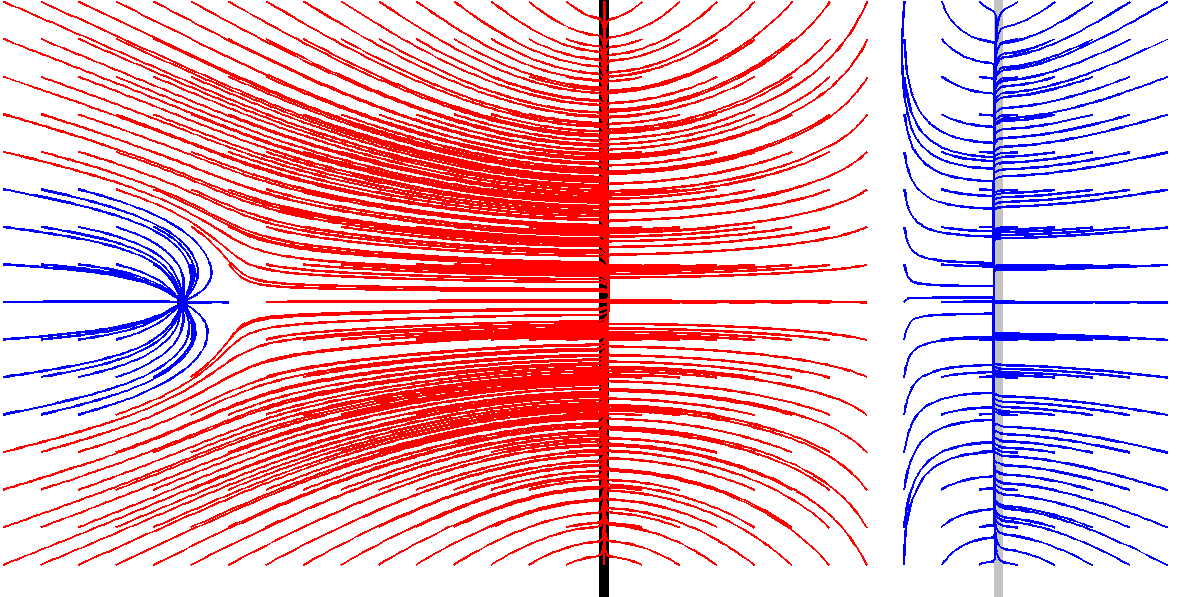
\includegraphics[scale=0.35]{Chapters/Images/m1_gamma_20.png}
     \caption{$\gamma=2.0$}
   \end{subfigure}
   \begin{subfigure}[c]{.5\linewidth}
     \centering
     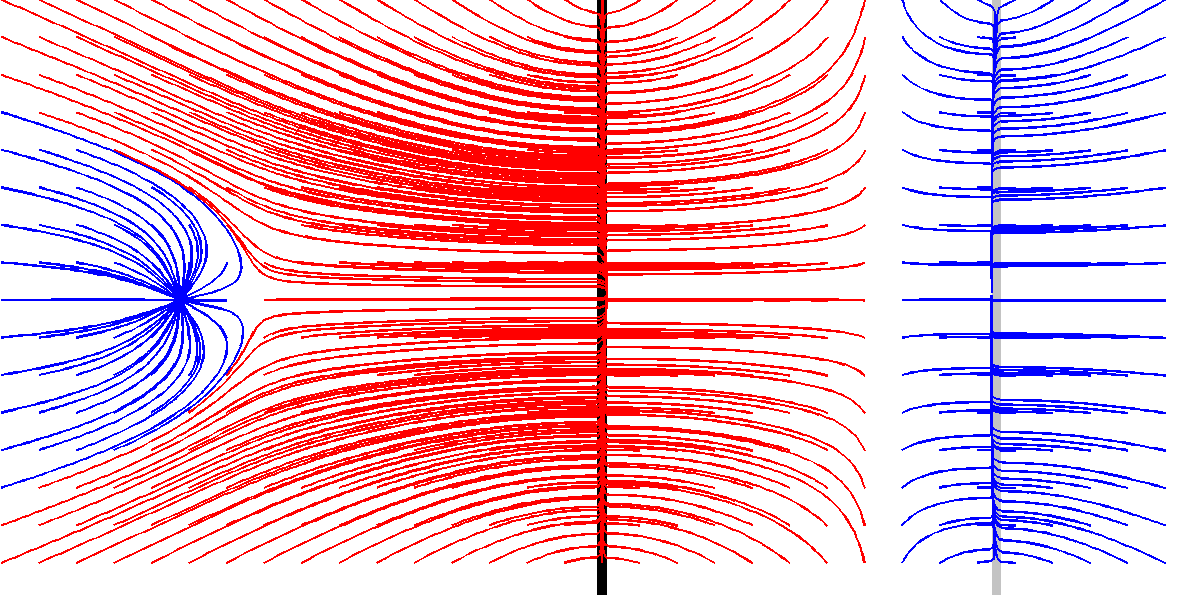
\includegraphics[scale=0.35]{Chapters/Images/m1_gamma_25.png}
     \caption{$\gamma=2.5$}
   \end{subfigure}\\
   
   \caption{(a) Carte de contours $F(x,y)$ synthétique avec un bruit impulsionnel, un contour fort et un contour faible. Lignes de courant générées à partir du champ VFC utilisant $m_1(x,y)$ avec plusieurs valeurs du paramètre $\gamma$ et pour un rayon $R=128$ du noyau de convolution.}
   \label{fig:gamma}
\end{figure}
\subsection{Analyse de $m_1(x,y)$}
\begin{figure}[!h]
   \begin{subfigure}[c]{.5\linewidth}
     \centering
     
\includegraphics[width=\textwidth]{Chapters/Images/synthetic_map.png}
     \caption{}
   \end{subfigure} 
      \begin{subfigure}[c]{.5\linewidth}
     \centering
     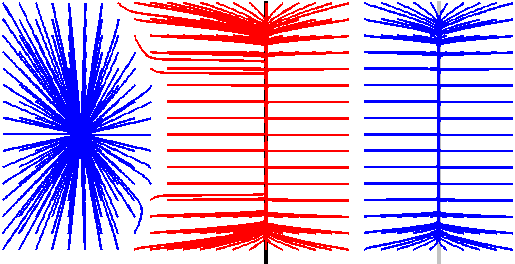
\includegraphics[width=\textwidth]{Chapters/Images/m2_sigma_10.png}
     \caption{$\sigma=10$}
   \end{subfigure} \\
   
   \begin{subfigure}[c]{.5\linewidth}
     \centering
     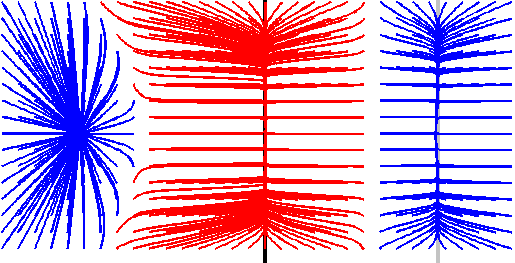
\includegraphics[width=\textwidth]{Chapters/Images/m2_sigma_15.png}
     \caption{$\sigma=15$}
   \end{subfigure}   
   \begin{subfigure}[c]{.5\linewidth}
     \centering
     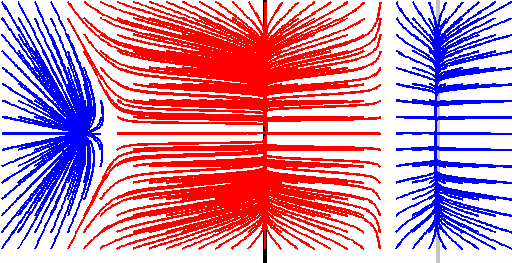
\includegraphics[width=\textwidth]{Chapters/Images/m2_sigma_20.png}
     \caption{$\sigma=20$}
   \end{subfigure}\\
   
   \begin{subfigure}[c]{.5\linewidth}
     \centering
     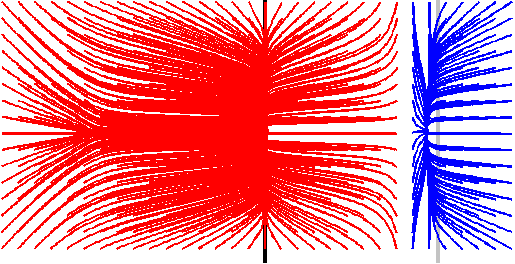
\includegraphics[width=\textwidth]{Chapters/Images/m2_sigma_25.png}
     \caption{$\sigma=25$}
   \end{subfigure}
   \begin{subfigure}[c]{.5\linewidth}
     \centering
     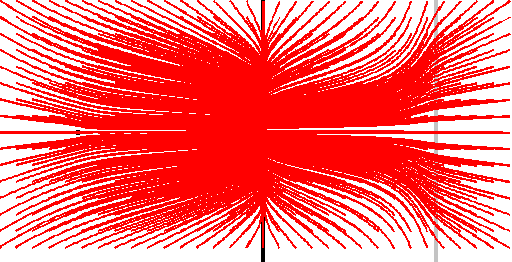
\includegraphics[width=\textwidth]{Chapters/Images/m2_sigma_30.png}
     \caption{$\sigma=30$}
   \end{subfigure}\\
   
   \caption{(a) Carte de contours $F(x,y)$ synthétique avec un bruit impulsionnel, un contour fort et un contour faible. Lignes de courant générées à partir du champ VFC utilisant $m_2(x,y)$ avec plusieurs valeurs du paramètre $\sigma$ et pour un rayon $R=128$ du noyau de convolution.}
   \label{fig:sigma}
\end{figure}